\chapter{Implementation}
\label{sec:implementation}

% Hier greift man einige wenige, interessante Gesichtspunkte der Implementierung
% heraus. Das Kapitel darf nicht mit Dokumentation oder gar Programmkommentaren
% verwechselt werden. Es kann vorkommen, daß sehr viele Gesichtspunkte
% aufgegriffen werden müssen, ist aber nicht sehr häufig. Zweck dieses Kapitels
% ist einerseits, glaubhaft zu machen, daß man es bei der Arbeit nicht mit einem
% "Papiertiger" sondern einem real existierenden System zu tun hat. Es ist
% sicherlich auch ein sehr wichtiger Text für jemanden, der die Arbeit später
% fortsetzt. Der dritte Gesichtspunkt dabei ist, einem Leser einen etwas
% tieferen Einblick in die Technik zu geben, mit der man sich hier beschäftigt.
% Schöne Bespiele sind "War Stories", also Dinge mit denen man besonders zu
% kämpfen hatte, oder eine konkrete, beispielhafte Verfeinerung einer der in
% Kapitel 3 vorgestellten Ideen. Auch hier gilt, mehr als 20 Seiten liest
% keiner, aber das ist hierbei nicht so schlimm, weil man die Lektüre ja einfach
% abbrechen kann, ohne den Faden zu verlieren. Vollständige Quellprogramme haben
% in einer Arbeit nichts zu suchen, auch nicht im Anhang, sondern gehören auf
% Rechner, auf denen man sie sich ansehen kann.

In the following section, I will explain some technical implementation details.
In particular, I want to highlight some of the implementation details of
components explained in chapter~\ref{sec:design}. First, I will refer to Linux,
which I use as the host kernel in the system. A special configuration was used
because I will make it run in parallel to the TEE kernel. Next, in
section~\ref{sec:implementation:teeKernel}, I will introduce phipsboot, which I
use as the TEE kernel, along with the modification I introduced to adapt it to
my use case. Another component I programmed is the Linux kernel module, which I
explain in section~\ref{sec:implementation:kmod}. In the last part of the
implementation chapter, I will explain how I implemented the attack simulations.

\section{TEE Kernel: phipsboot}
\label{sec:implementation:teeKernel}

PhipsBoot is a Multiboot 2 compliant kernel mainly written in the memory-safe
programming language Rust, which is designed to be relocatable in the memory. It
depends on a first-stage bootloader\todo{maybe this is not a multi-stage
    bootloader} that brings the system to a state defined in the Multiboot 2
specification. That is, the CPU is in 32-bit mode with segmentation enabled.
After handover, PhipsBoot does all initialization steps to bring the CPU into
64-bit with enabled PEA paging. It initializes the page tables and sets up huge
pages for the initial mapping. PhipsBoot expects to be loaded to a 2 MiB-aligned
address. Its small size, which is less than 2 MiB, allows PhipsBoot to set up
the page table hierarchy using a single page table that maps the kernel.
PhipsBoot uses memory statically reserved for dynamic memory allocation in the
kernel's Elf image. Next to being relocatable, PhipsBoot does not implement more
features but offers a great starting point for implementing the TEE features. \\

The first feature I introduced was modifying page tables. This feature was
lacking because PhipsBoot's purpose does not require the modification of the
page to map, for example, mapping memory that is not contained in its binary.
For this, I modified the page table setup routine and changed the last page
table to be writable instead of read-only. Through observation, I found that not
more than the first 128 entries in the page table are used to map all kernel
memory. For dynamic mapping, I, therefore, reserved the last 128 entries. This
enabled PhipsBoot to map memory that was not contained in the binary. This
feature is important to implement the shared memory communication path. The
address is communicated to PhipsBoot through the Multiboot 2 memory map. To
access this structure, PhipsBoot needs to be able to map the page containing it.
Moreover, the address in the memory map must be mapped by PhipsBoot to make the
shared memory accessible. Other than the memory owned by the kernel, the memory
intended to be used by the TEE kernel and the host kernel is mapped as
uncacheable. This prevents cache pollution and false positives for allowed
access of a remote core to memory, also used by the TEE.\\

To prepare the environment, the TEE kernel needs to ensure that all memory used
by it is in the exclusive or modified state so that a remote core must trigger
an offocre\todo{Irgendwo mal erklären was ein OFfcore event ist} event when it
tries to access memory owned by the TEE kernel. For this, I implemented a
function that iterates over the page table entries and copies all bytes in
place. This triggers the modified state of the cache line, which leads to
invalidating the cache line in remote cores referencing the same memory item. I
discovered this necessity when implementing my attack simulations
(c.f.~\ref{sec:implementation:attacks:memory}). While the TEE could detect the
active attacker, the passive one was undetectable because the reading of cache
lines, which are in the shared state in both caches, does not trigger any
microarchitectural responses. It is, therefore, necessary to hold all memory
that the TEE should keep secret in the exclusive or modified state to detect
cache synchronization over the cache coherency protocol.\\

After ensuring that all attempts to manipulate or access secret memory do not
result in additional microarchitectural state changes, it is time to make the
TEE detect the respective events resulting from access to the remote core
through monitoring performance counters. For this, the TEE writes the respective
events to the configuration MSRs. Once prepared, the TEE sets the IDTR to null,
which leads to triple faulting once an interrupt is delivered to the TEE. The
only expected interrupts in the TEE are NMIs, PMIs, and IPIs from other cores.
All other interrupts are masked by clearing the interrupt flag in the EFLAGS
register of the isolated core. \\

NMIs can be sent by faulty hardware and the interrupt controller if configured
accordingly. Currently, the TEE has no other means of defense against malicious
SMM code. IPIs originate from other cores and can be sent by those at any time.
Because IPIs are routed through the IDT, the same countermeasures as with NMIs
are taken. The invalid setting of the IDTR to NULL results in a triple fault
that ultimately results in a reset of the whole machine. The same defense
strategy is employed upon registering an offshore event triggered through a
read-or-write attempt from a remote core. By defining a threshold for event
occurrence upon which overflow emits a PMI, the TEE can terminate as it wishes.
A useful threshold is 1, which results in a PMI triggered by the first
occurrence of the respective event. For this, we use an event that counts all
occurrences of off-core communication not served by main memory. This works
because all memory is placed in the cache, and only the communication routine is
accessing the uncacheable main memory. \\

\begin{center}
    \begin{figure}
        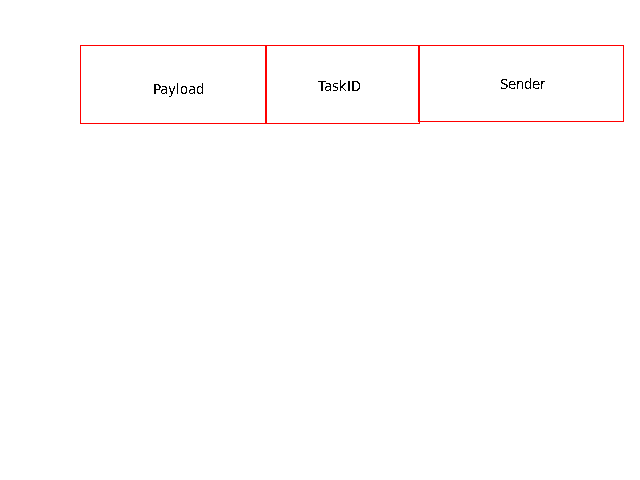
\includegraphics[width=0.8\textwidth]{images/shared_mem_placeholder.png}
        \caption{Shared memory protocol}
        \label{fig:shared-mem}
    \end{figure}
\end{center}
\todo{replace graphic}

I implemented a structure to manage the memory in question to enable
communication through the shared memory channel. Access to the shared memory
follows a simple protocol that splits the memory, as shown in
figure~\ref{fig:shared-mem}. The first byte denotes the sender, the second
denotes the task identifier, and the remaining part is used for a payload that
can be sent along with the other tags. I assume there are only two communication
parties in the current prototype: the TEE kernel and the host kernel. A message
is sent by writing the first byte. To receive a message, the respective party
polls the first byte of the shared memory and waits until the signal is written
by the other party, \\

After initialization, the TEE environment starts a state machine that controls
the execution of tasks. In the first state, the TEE polls the shared memory
until it receives a message containing the command to execute one of the
predefined tasks. Once this message is received, the TEE executes the task as
commended. While the task runs, it can access the shared memory for multiple
reasons. The first reason is that the task can access the payload section of the
memory to receive additional input data from the party outside of the TEE. The
second reason is that the task can prepare an answer to the third-party request.
For this, the task can write to the sender information, the command, and the
payload fields as it wishes. It is the task's responsibility to write to the
shared memory data needed to create a response to the request once it is done.
After the task returns, the TEE creates a report from the performance counters
and sends the result to the third party over the shared memory
channel.\todo{Does it really?} \\

\section{Host Kernel: Linux}
\label{sec:implementation:hostKernel}

As a highly configurable open-source general-purpose operating system, Linux is
an example of the implementation of the host kernel. The Linux kernel I used for
my prototype is version 6.13. Linux allows the configuration at runtime by
passing command line arguments to the kernel on boot. This makes it able to
limit the resources Linux uses. \\

To isolate the CPU core, I used the command line option \textit{nr\_cpus=n},
where $n$ is an arbitrary number that limits Linux from using a maximum core
count of $n$. I used $n=3$ to limit Linux to 3 cores. While Linux supports CPU
hotplugging\todo{ref}, which would allow enabling core to be turned off through
the same feature, \textit{nr\_cpu} introduces a hard limit. Thus, cores excluded
from initialization by this parameter are inaccessible for Linux and can't be
hotplugged later. \\

Another useful parameter is \textit{memmap}, which I used to add custom entries
to the BIOS memory map that Linux uses to set up its memory map. With this, I
added an entry with type \textit{persistent} of 4KiB size starting at the
address $0x9000$ is within the first MiB of system memory and not marked free in
the BIOS specification\todo{cite}. I reserve this memory in order to use it
later for booting one of the excluded CPUs, as x86 CPUs initialize in 16-bit
mode and, therefore, can only access memory with addresses lower than the 1 MiB
boundary. Linux does not offer any procedure to allocate memory in this address
region, so this is the only possible way. \\

Other preparation steps are done by the Linux kernel module explained in
section~\ref{sec:implementation:kmod}. Linux Neverthelss serves is the first
software to be run in my prototype. All other components, namely the TEE kernel
as an Elf-file image and the Linux kernel module, are embedded in its initial
RAM disk image, which allows, in theory, to sign a single image for secure boot
and thus ensure the integrity of all components on startup.\\

\section{Linux kernel module}
\label{sec:implementation:kmod}
As I described in section~\ref{sec:implementation:hostKernel}, the Linux kernel
module is the driver not only enabling Linux to communicate with the TEE kernel
on the isolated core but also the component that initializes the isolated core
and loads the TEE kernel into memory.\\

For this, the kernel module claims the memory reserved through the Linux command
line argument and copies the startup code. This code sequence brings the
processor from real mode into 32-bit mode with segmentation and places the
addresses of Multiboot 2 structures into the registers. The resulting state is
the one expected by the TEE kernel. Because these addresses are not known
beforehand, the kernel module modifies the startup code on runtime to contain
the respective addresses.\\

In the next step, the kernel module locates the Elf binary of the TEE kernel and
places it in memory. For this, the module allocates memory through the Linux
kernel's \textit{allocpages} interface at a physical address aligned to 2 MiB.
Once allocated, the kernel module does not deallocate the pages to prevent Linux
from reusing the memory and possibly overwriting the TEE kernel. Once the
required memory is allocated and mapped in the kernel address space, the kernel
module begins to parse the TEE kernel's Elf image and copies all necessary parts
to memory. It then sets up the shared memory region and updates. It generates a
multiboot 2 Information structure containing the region with a custom-defined
memory type used by the TEE kernel to find the shared memory.\\

Once all parts necessary to run the TEE kernel are placed in memory, the kernel
module prepares to start the isolated core. At this point, Linux does not allow
interaction with any core not initialized by it, e.g., the kernel module cannot
address the isolated core with any kernel-provided functions. To circumvent this
shortcoming, I gained access to the LAPIC of the core running the kernel module
to send the required INIT and startup IPI sequence to the isolated core. Another
problem arises when implementing this routine: APIC IDs are not bound to start
at 0, nor do they have to increment by one for each CPU core. To come by this, I
queried the APIC IDs of the core mapped by Linux and calculated the offset for
each core. I used this offset to calculate the APIC ID of the target core by
adding the offset to the ID of the last core mapped by Linux. After sending the
IPI sequence to the remote core, the startup code will be executed, and a far
jump to the TEE kernel's code will be performed by the remote CPU.\\

After initializing the remote core, the kernel module manages communication with
the TEE kernel. It therefore implements the protocol described in
\ref{sec:implementation:teeKernel}. To receive messages, the kernel module
installs a timer, which it uses to poll the shared memory periodically for new
messages. The kernel module also implements the remote part of tasks in the
prototype. To start a specific task, the kernel module sends a message
containing the task's ID and evaluates messages from the TEE to delegate them to
the respective tasks routine. \\
\todo{If anything ever uses the chardev then I should write about it}

\section{Attacks and Applications}
\label{sec:implementation:attacks}

To proof the effectiveness of the prototype I implemented three possible attacks
as tasks. Furthermore, I impemented a simple \textit{ping} task that allows me to
investigate ressource usage of the TEE allone. In the follwing subsection I want
to show some implementationt details of the attacks and the \textit{ping} taks.

\subsection{Ping Task}
\label{sec:implementation:attacks:ping}
This simple task does nothing more than to increment a value shared between the
TEE and the host OS. It can be viewed as the minimal working set of the TEE to
run tasks. Therefore, the result for memory usage is the minimum to expect for
any other task. Measuring the resource usage with appropriate PMC allows me to
make assumptions about the resources a future payload can use. I collected data
with the following events:
\begin{itemize}
    \item L1 replacements
    \item L1 Miss (any)
    \item Offcore events \todo{umask and so angeben um reproduzierbarkeit zu
              wahren}
\end{itemize}
Between each ping cycle I used used the \textit{wbinvd} instruction of x86, that
results in the core writing back all it's cache entries to memory and
invalidating each cache line. Executing the following ping cycle until reading
the PMC again yields the number of cache lines filled with data necessary to
execute a complete cycle. From the cache line size I can then conclude the total
memory requirements of the runtime part of the TEE.

\subsection{Stalling Attack}
The denial of service attack floods the TEE with NMIs. It is intended to prove
that the TEE can defend against interrupts that the TEE cannot mask.
\todo{maybe move this into the chapter intro}


\subsection{Memory Attacks}
\label{sec:implementation:attacks:memory}
In theory, an attacker is able to leak data through the microarchitectural
behavior of the CPU cache's implementation. The first attacker is passive and
only interested in spying unobserved on the secrets of the TEE. The attacker
would use their access to read the TEE memory. If the TEE cannot observe this,
then secrets could be leaked through this channel upon writing. The second
attacker is an active one who tries to write the TEE memory to influence its
control flow. Both attacks follow the same workflow.\\

To simulate these attacks, the TEE first initializes a memory area of the size
of 4KiB and finds its physical location. Because I want to observe the side
effects of the attack, this memory is not mapped as uncacheable on the TEE side
but instead like any other memory in the TEE. The TEE then communicates the
address through the shared memory channel to the Linux kernel module in which
the respective attack implementations reside. The remote side now maps the
physical address space into its address space and either reads or writes to the
memory. When finished, the remote kernel module creates the respective answer
and transfers control over the memory area on this way back to the TEE. The TEE
now reports on the state of the performance counters.\todo{maybe add some code
    examples?}\\

\cleardoublepage

%%% Local Variables: %% TeX-master: "diplom" %% End:
